\section{Amplificatore operazionale}

\begin{defn}[Generatori dipendenti]
    Un generatore dipendente è un elemento che genera una grandezza elettrica (tensione o corrente) il cui valore è funzione di
    un'altra grandezza elettrica (tensione o corrente) presente nel circuito.
    I generatori dipendenti sono “doppi bipoli”, cioè hanno una coppia di terminali di ingresso per la variabile di controllo e 
    una coppia di terminali di uscita per la grandezza generata. 
    Convenzionalmente, nelle figure i terminali di ingresso sono a sinistra e i terminali di uscita sono a destra.
\end{defn}

\begin{defn}[Generatore di tensione controllato in tensione]
	All'ingresso non assorbe corrente (si comporta come un circuito aperto).\\
	Il parametro $E$ è il guadagno di tensione (adimensionale): $E = V_o / V_i$
	\begin{figure}[H]
		\centering
		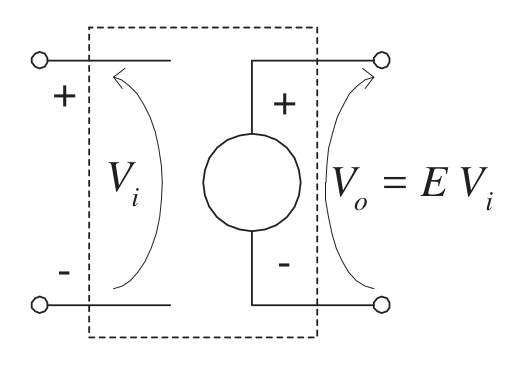
\includegraphics[width=0.5\linewidth]{figures/VCVS.png}
		\caption{VCVS}
		\label{fig:VCVS}
	\end{figure}
\end{defn}

\begin{defn}[Generatore di corrente controllato in corrente]
	All'ingresso non c'è caduta di tensione (si comporta come un cortocircuito). \\
	Il parametro $F$ è il guadagno di corrente (adimensionale): $F = I_o / I_i$
	\begin{figure}[H]
		\centering
		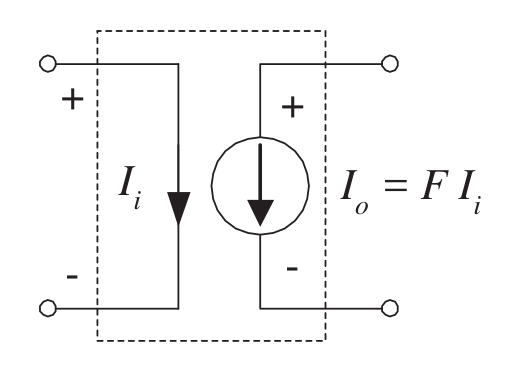
\includegraphics[width=0.5\linewidth]{figures/CCCS.png}
		\caption{CCCS}
		\label{fig:CCCS}
	\end{figure}
\end{defn}

\begin{defn}[Generatore di corrente controllato in tensione]
	All'ingresso non assorbe corrente (circuito aperto). \\
	Il parametro $G$ è la transconduttanza, o conduttanza di trasferimento tra ingresso e uscita, che dimensionalmente è una conduttanza e si misura in Siemens:
	$G = I_o / V_i$
	\begin{figure}[H]
		\centering
		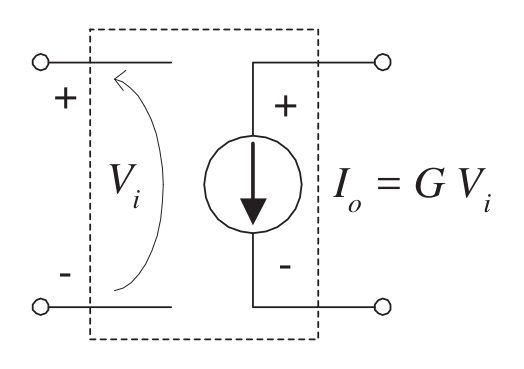
\includegraphics[width=0.5\linewidth]{figures/VCCS.png}
		\caption{VCCS}
		\label{fig:VCCS}
	\end{figure}
\end{defn}

\begin{defn}[Generatore di tensione controllato in corrente]
	All'ingresso non c'è caduta di tensione (cortocircuito). \\
	Il parametro $H$ è la transresistenza o resistenza di trasferimento tra ingresso e uscita, che dimensionalmente è una resistenza e si misura in Ohm:
	$H = V_o / I_i$
	\begin{figure}[H]
		\centering
		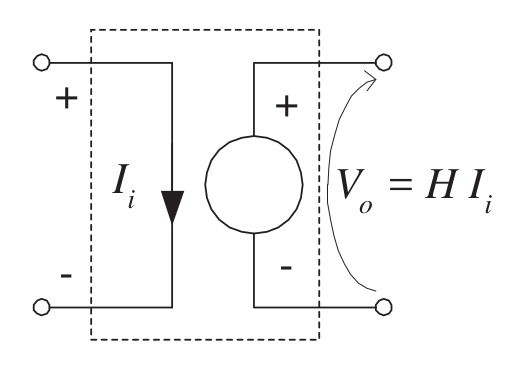
\includegraphics[width=0.5\linewidth]{figures/CCVS.png}
		\caption{CCVS}
		\label{fig:CCVS}
	\end{figure}
\end{defn}

